\section{Experteninterview} \label{Experteninterview}
Heutzutage ist die Bedeutung von Experteninterviews in der Forschungspraxis unumstritten. In verschiedensten Bereichen gehört es fest zum Kernbestand der alltäglichen Forschungsroutine, sei es als eigenständige Erhebungsmethode oder als ergänzende Methode im Rahmen explorativer Forschung. \footcite[Vgl.][S. 1]{Bogner_2014_Interview}

% Wesentliche Funktionen des Experteninterviews sind Informationsgewinnung und Theorieentwicklung, weswegen es sich als Methode eignet, um Anforderungen zu erheben.
% \footcite[Vgl.][S. 187 f.]{Glaeser_2010_Inhaltsanalyse}$^,$\footcite[Vgl.][S. 9]{Bogner_2014_Interview}
%
% Wenn von Experteninterviews die Rede ist, kann man davon ausgehen, dass ein leitfadengestütztes, qualitatives Interview gemeint ist. Da das Instrument Experteninterview dem Forschungsvorhaben angepasst werden muss, können jedoch verschiedene Dinge unter dem Begriff verstanden werden und es ist nötig klarzustellen, welche Ausprägung gemeint ist.\footcite[Vgl.][S. 3]{Bogner_2014_Interview}
% Auch der Expertenbegriff muss der Forschungsfrage angepasst werden.\footcite[Vgl.][S. 180]{Meuser_1994_Interview}

% In dieser Arbeit wird ausschließlich der qualitativ ausgerichtete Ansatz von Meuser und Nagel verfolgt. Quantitative Ansätze oder qualitative Ansätze anderer Autoren, die von dem behandelten abweichen werden hier nicht weiter ausgeführt.\footcite[Vgl.][o.S.]{Meuser_2010_Interview}

% Um das Experteninterview anwenden zu können, muss geklärt werden, wer als Experte gilt, was Expertenwissen bedeutet und wie man es abruft, welche Schritte zur Vorbereitung eines Interviews erforderlich sind, welche Gesprächsführung für die Forschungsfrage Sinn macht und wie die Interviews ausgewertet werden können.\footcite[Vgl.][S. 6 f.]{Bogner_2014_Interview}


% \subsection{Arten}
% Meuser und Nagel unterscheiden Experteninterviews grundlegend in systematisierende und explorativ-felderschließende Interviews. Bei ersteren wird der Experte zu seinem eigenen Fachgebiet befragt (Betriebswissen), bei letzerem liefert er lediglich \glqq{}Informationen über die Kontextbedingungen des Handelns der Zielgruppe\grqq (Kontextwissen)\footcite[][S.445]{Meuser_1991_Interview} .
%
% Bogner, Littig und Menz sprechen in diesem Zusammenhang von fundierenden und explorativen Interviews und fasst die vormals genannten Kategorien unter dem Begriff \textit{informatorisch} zusammen. Außerdem ergänzt er zwei  deutungswissenorientierten Varianten. Eine genaue Aufschlüsselung ist in \autoref{tab:artenei} zu sehen.\footcite[Vgl.][S. 445 f.]{Meuser_1991_Interview}$^,$\footcite[Vgl.][S. 22 ff.]{Bogner_2014_Interview}
%
%
% \begin{table}[H]
% \centering
% \begin{tabularx}{1\textwidth}{XXX}%
%                             & Explorativ (Kontextwissen) & Fundierend (Betriebswissen) \\\midrule
%    Informatorisch           & Explorative Datensammlung & Systematisierendes Interview \\
%    Deutungswissenorientiert & Exploration von Deutungen & Theoriegenerierendes Interview
% \end{tabularx}
%   \\\quelle{Bogner_2014_Interview}
%   \\\quelle{Meuser_1991_Interview}
% \caption{Arten von Experteninterviews}
% \label{tab:artenei}
% \end{table}


\subsection{Phasen}
% Ein Experteninterview kann aus bis zu acht Phasen bestehen, diese sind in \autoref{tab:phasenei} aufgeführt und anschließend im Detail erläutert. Für die Abfrage von Betriebswissen müssen alles Phasen durchlaufen werden, bei Kontextwissen entfallen die letzten beiden.\footcite[Vgl.][S. 466 f.]{Meuser_1991_Interview}

\begin{table}[ht]
\centering
\begin{tabularx}{1\textwidth}{llX}%
Nr. & Phase                            & Aktivitäten \\\midrule
1   & Leitfadenerstellung              & Erstellung des Leitfadens\\
2   & Tonaufnahme                      & Aufzeichnung des Gesprächs\\
3   & Transkription                    & Übertragung in Schriftdeutsch\\
4   & Paraphrase                       & Zusammenfassung und thematische Einteilung\\
5   & Überschriften                    & Verdichtung, Betitelung der paraphrasierten Abschnitte\\
6   & Thematischer Vergleich           & Vergleich aller Intervews, Suche nach Gemeinsamkeiten\\
7   & Soziologische Konzeptualisierung & Systematisierung, Typisierung, Deutung \\
8   & Theoretische Generalisierung     & Bildung von Theorien, Interpretation der Ergebnisse
\end{tabularx}
  \\\quelle{Meuser_1991_Interview}
\caption{Phasen eines Experteninterviews}
\label{tab:phasenei}
\end{table}

% \subsubsection{Transkription}
% Das Hauptaugenmerk von Experteninterviews liegt auf der Gewinnung von Wissen. Daher ist eine mühselige Notation, wie sie bei narrativen Interviews vorgenommen wird nicht nötig. Elemente wie Pausen, Betonung oder Stimmlage werden nicht interpretiert.
% Eine Transkription wird in der Regel nicht für die gesamte Tonaufnahme durchgeführt, sondern kann selektiv erfolgen. Bei der Abfrage von Betriebswissen fällt die Transkription umfangreicher aus als bei Kontextwissen. \footcite[Vgl.][S. 455 f.]{Meuser_1991_Interview}
%
% \subsubsection{Paraphrase}
% Die Paraphrase erfolgt unter Berücksichtigung der Forschungsfrage und gibt die Aussagen der Experten chronologisch geordnet und unverfälscht wieder, wobei diese zu thematischen Verbünden zusmamengefasst werden. Ob die Passage zusammenfassend oder detailliert wiedergegeben wird hängt von der Priorität des Themas und nicht zwangsläufig von der ihm gewidmeten Zeit ab.\footcite[Vgl.][S. 456 f.]{Meuser_1991_Interview}
%
% \subsubsection{Überschriften}
% Die paraphrasierten Abschnitte werden möglichst textnah mit einer oder mehreren Überschriften versehen, je nach dem, wie viele Themen angesprochen werden. Dabei ist darauf zu achten, dass das Expertenwissen im Fokus steht, der Experte als Person ist nicht relevant.\footcite[Vgl.][S. 458 f.]{Meuser_1991_Interview}

% \subsubsection{Thematischer Vergleich}
% Ab diesem Schritt werden nicht mehr die Interviews im Einzelnen betrachtet, es erfolgt ein Vergleich der thematisch ähnlichen Textpassagen aller Interviews, wobei die Überschriften nach Möglichkeit vereinheitlicht werden. Es wird geprüft, ob sich die Äußerungen der Experten decken oder ob sie unterschiedliche Ansichten haben. Außerdem wird betrachtet, zu welchen Themen sich alle Experten äußern und zu welchen nur einzelne.\footcite[Vgl.][S. 459 f.]{Meuser_1991_Interview}$^,$\footcite[Vgl.][S. 37]{Matthes_1986}
%
\subsubsection{Soziologische Konzeptualisierung}
In diesem Schritt werden aus dem gemeinsamen Wissen der Experten Kategorien gebildet, wodurch eine weitere Verdichtung des Wissens erfolgt. Dadurch soll eine Typisierung, Verallgemeinerung und Deutung des Wissens möglich werden. Die Struktur des Expertenwissens wird betrachtet, wodurch die Reichweite der Konzepte geprüft werden kann.\footcite[Vgl.][S. 462 f.]{Meuser_1991_Interview}

\subsubsection{Theoretische Generalisierung}
Im letzten Schritt werden Theorien aus Sinnzusammenhängen gebildet und die Ergebnisse interpretiert, wobei darauf zu achten ist, dass man sich nicht von Verdachten leiten lässt, sonder nur mit dem Forschungsmaterial arbeitet.\footcite[Vgl.][S. 463 ff.]{Meuser_1991_Interview}




\subsection{Definition: Experte}
% Das Wort \textit{Experte} leitet sich aus dem lateinischen \textit{expertus} (erprobt, bewährt) ab, welches wiederum aus dem passiven Verb \textit{experiri} (prüfen, ausprobieren) gebildet wird. Experten sind also Fachleute und Kenner, bzw. allgemein gesprochen Personen, die über ein gewisses Spezialwissen verfügen, das auf der Erfahrung des ausgiebigen Prüfens und Ausprobierens fußt. \footcite[Vgl.][S. 9]{Bogner_2014_Interview}
%
% Wie in \autoref{fig:experte} zu erkennen, zeichnet sich ein Experte durch eine bestimmte Kombination von Macht und Wissen aus, welche ihn von Eliten, Spezialisten und spezialisierten Laien unterscheidet.\\ \glqq{}Der Experte ist -- im Gegensatz zum Spezialisten – nicht allein durch Sonderwissen in Form fachspezifischer Kompetenzen charakterisiert, sondern durch seine Fähigkeit, Verbindungen zu anderen Wissensbeständen und Wissensformen herzustellen und die Relevanz des eigenen Wissens zu reflektieren\grqq. \footcite[][S. 14]{Bogner_2014_Interview}$^,$\footcite[Vgl.][S. 21 f.]{Hitzler_1994}
%
% \begin{figure}[H]
%   \centering
%   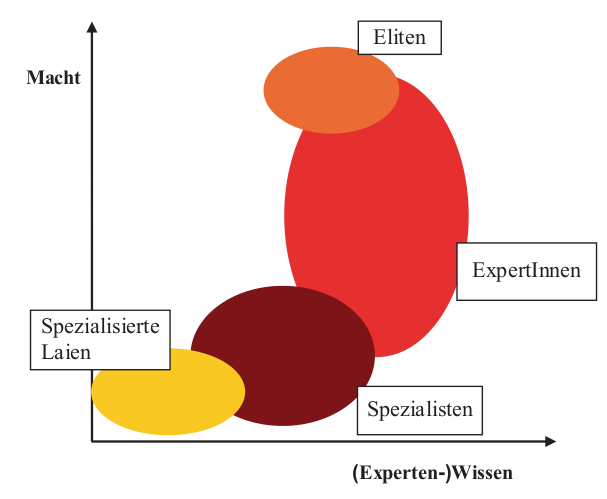
\includegraphics[width=0.6\textwidth]{Anhang/Experte}
%   \\\quelle{Littig_2008}
%   \caption{Experteneinordnung}
% \label{fig:experte}
% \end{figure}
%
% Gläser und Laudel definieren Experten als Menschen, die ein besonderes Wissen über soziale Sachverhalte besitzen.\footcite[Vgl.][S. 12]{Glaeser_2010_Inhaltsanalyse} Man könnte nun davon ausgehen, dass jeder ein Experte ist, da er sich in seinem Fachgebiet gut auskennt. Genauer betrachtet  gibt es jedoch große Unterschiede zwischen Laien und Experten, man bedenke nur das Verhältnis zwischen Ärzten und Patienten. Ein solcher Expertenbegriff ist also zu weit gefasst und es kann nicht jedes qualitative Interview automatisch als Experteninterview bezeichnet werden.\footcite[Vgl.][S. 10 f.]{Bogner_2014_Interview}
%
% Meuser und Nagel hingegen betrachten den Experten als Konstrukt des Forschungsinteresses. Die Expertise ist also keine allgemeingültige Eigenschaft oder Fähigkeit einer Person, sondern eine Zuschreibung des Forschenden an diese, im speziellen Kontext der Forschungsfrage. \footcite[Vgl.][S. 181]{Meuser_1994_Interview}
%


\subsection{Definition: Expertenwissen}
Als einer der ersten hat Schütz das Expertenwissen als sicheres und eindeutiges Wissen beschrieben, das dem Experten \glqq{}jederzeit kommunikativ und reflexiv\grqq\footcite[][S. 12]{Bogner_2014_Interview} verfügbar ist.\footcite[Vgl.][S. 86 ff. ]{Schuetz_1972}
Sprondel ergänzte anschließend, dass das Expertenwissen komplex integrierte Wissensbestände umfasst und auf den professionellen Funktionskontext bezogen ist.\footcite[Vgl.][S. ]{Sprondel_1979}

Expertenwissen spielt in der modernen Gesellschaft eine wichtige Rolle in allen Lebensbereichen, nicht nur in der Wissenschaft. Z. B. Fragen der Gesundheit oder Ernährung werden nicht intuitiv entschieden, sondern auf Basis von Expertise. Dieser Umstand stellt zwar eine Abhängigkeit dar, trägt jedoch dazu bei, dass unsere heutige Gesellschaft eine Wissensgesellschaft mit starker Spezialisierung ist.\footcite[Vgl.][o.S.]{Coser_1992}$^,$\footcite[Vgl.][S. 10]{Bogner_2014_Interview}
% \todo{Seite suchen: Giddens1991}
Umgekehrt betrachtet stellte Nowotny fest, dass die Expertise heutzutage nicht nur in der Wissenschaft, sondern in allen Bereichen der Gesellschaft gebildet wird.\footcite[Vgl.][S. 215 ff. ]{Nowotny_2001}$^,$\footcite[Vgl.][S. 10]{Bogner_2014_Interview}
%
% Das Interessante am Expertenwissen ist nicht nur das Wissen an sich, sondern die Wirkung in der Praxis. Experten werden gefragt, weil ihre Entscheidungen und Ratschläge das Handeln anderer Akteure mitstrukturieren und -gestalten.\footcite[Vgl.][S. 13]{Bogner_2014_Interview} Bogner spricht davon, dass Expertenwissen \glqq seine Bedutung über [...] soziale Wirkmächtigkeit\grqq{} erhält.\footcite[][S. 13]{Bogner_2014_Interview}
% Ferner folgert er daraus die Definition:\\ \glqq Experten lassen sich als Personen verstehen, die sich -- ausgehend von einem spezifischen Praxis- oder Erfahrungswissen, das sich auf einen klar begrenzbaren Problemkreis bezieht -- die Möglichkeit geschaffen haben, mit ihren Deutungen das konkrete Handlungsfeld sinnhaft und handlungsleitend für Andere zu strukturieren.\grqq{}\footcite[][S. 13]{Bogner_2014_Interview}
%

% \subsection{Vorbereitung des Interviews}
%   \todo{Erstellung des Leitfadens}
% \subsection{Wahl der Gesprächsführung}
% \subsection{Auswertung der Interviews}
%
% \footcite[Vgl.][S. 448 f.]{Meuser_1991_Interview}
%   \todo{Auswertung, Transkription, Paraphrase, Überschriften, Theoretischer Vergleich,}
%

% \footcite[Vgl.][o. S.]{Burger_2011_Interview}
